% Nicholas M. Rathmann <rathmann@nbi.ku.dk>

\documentclass[border=1pt,tikz]{standalone}

\usepackage{pgfplots,physics}
\usepackage{newtxtext,newtxmath} % RSPA-like font
\usetikzlibrary{calc,arrows.meta,decorations.markings}

\usepackage{xcolor}

\definecolor{dblue}{HTML}{08519c}
\definecolor{dred}{HTML}{a50f15}

\definecolor{cray1}{HTML}{542788}
\definecolor{cray2}{HTML}{b35806}

\definecolor{cice}{HTML}{dcf0fd}
\definecolor{cbed}{HTML}{c9b1a2}

\tikzstyle{iceshading}=[top color=cice!200, bottom color=cice!90]
\tikzstyle{bedshading}=[top color=cbed, bottom color=cbed!160]

\tikzset{
	every picture/.style={font=\fontsize{9.1}{9.1}\selectfont,},
	anno/.style={font=\fontsize{8.5}{8.5}\selectfont,},
  	lw/.style={line width=0.9pt,},
	%%%
  	bed/.style={black, bedshading},
  	bedtop/.style={black, lw},
  	icesheet/.style={dblue, iceshading},
	%%%
	CMPdot/.style={dred, fill=dred, lw}, 
	ray1/.style={lw, cray1},
	ray2/.style={lw, cray2},
	reflector/.style={dblue}, 
	axis/.style={black, lw, -{Latex[scale=0.9]}, line cap=rect,},
	decoration={markings, 
		mark=at position 0.32 with {\arrow{Latex[scale=1.1]}},
		mark=at position 0.64 with {\arrow{Latex[scale=1.1]}}
	},
}

\gdef\W{6cm}		% width
\gdef\H{2.6cm}		% ice thickness
\gdef\Hbed{0.5cm}	% bed thickness
\gdef\Hrfl{0.8cm}	% reflector level

\gdef\xT{\W/2 * 0.7}

\begin{document}
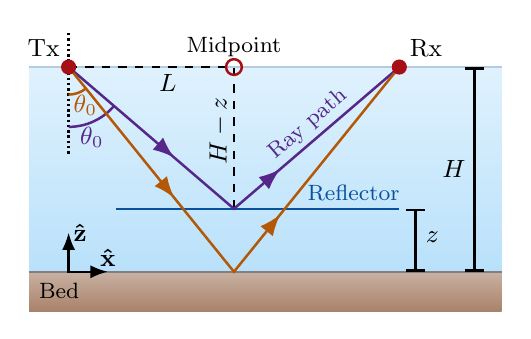
\begin{tikzpicture}[]

	%%% Ice, bed

	\begin{scope}[xshift=0.4cm]
	
		\fill[icesheet, shading angle=180] ({-\W/2},0) rectangle ++(\W,\H);
		\draw[lw, dblue!30] (-\W/2,\H) -- ++(\W,0);
		
		\fill[bed] (-\W/2,-1*\Hbed) rectangle ++ (\W,\Hbed);
		\draw[bedtop, black!50] (-\W/2,0) -- ++(\W,0);
		\node[anchor=west,anno] at (-1*\W/2,-0.7em) {Bed};

	\end{scope}

	\draw[dashed, lw] (0,\Hrfl) -- (0, \H) node[pos=0.55, xshift=0.2em, anchor=south, rotate=90] {$H-z$};

	\coordinate (P0) at (-\xT, \H);
	\coordinate (P2) at (\xT, \H);
	\coordinate (P1) at (0, \Hrfl);
	
	\begin{scope}[]
		\gdef\axlen{0.5cm}
		\coordinate (Pa) at ($(P0)-(0,\H)$);
		\draw[axis] (Pa) -- ++(0, \axlen) node[black,right=-0.2em] {$\vu{z}$};
		\draw[axis] (Pa) -- ++(\axlen, 0) node[black,above=-0.2em] {$\vu{x}$};

		\draw[lw, densely dotted, black] (P0) -- ++(0,  0.45cm);
		\draw[lw, densely dotted, black] (P0) -- ++(0, -1.13cm);
	\end{scope}

	%%% Reflector 
	
	\draw[lw, color=dblue] (-1*\W/2 * 0.5, \Hrfl) -- (\W*0.35, \Hrfl) node[anno, below, anchor=south east, pos=1, inner sep=0.25em, xshift=+0.3em] {Reflector};	

	%%% Rays

	\gdef\R{0.76cm}
	\draw[lw, ray1] (P0) ++(-90:\R) arc (-90:-40:\R) node[pos=0.2,inner sep=0,anchor=north west,] {$\theta_0$};
	
	\draw[ray1, postaction={decorate}] (P0) -- (P1) -- (P2) node[anno, pos=0.51, above=-0.15em, sloped] {Ray path};
	
	\coordinate (P1b) at (0, 0);
	\draw[ray2, postaction={decorate}] (P0) -- (P1b) -- (P2);

	\gdef\R{0.35cm}
	\draw[lw, ray2] (P0) ++(-90:\R) arc (-90:-50:\R) node[pos=0.2,inner sep=0,anchor=north west,] {$\theta_0$};

	%%%% Labels, dots, axes
	
	\draw[black, lw, dashed] (P0) -- (0,\H) node[pos=0.6, anchor=north, yshift=0.1em] {$L$};
	
	\draw[CMPdot] (P0) circle[radius=0.08cm] node[above left, black, inner xsep=0] {Tx\hspace*{0.3em}};
	\draw[CMPdot] (P2) circle[radius=0.08cm] node[above right, black] {Rx};
	\draw[CMPdot, fill=none] (0,\H) circle[radius=0.1cm] node[anno,above, black] {Midpoint};

	\draw[lw, |-|, xshift=0.5em] (\W*0.71/2,0) -- ++(0,\Hrfl) node[right,pos=0.55, anchor=west] {$z$};
	\draw[lw, |-|, xshift=0.5em] (\W*1.92/4,0) -- ++(0,\H) node[left=-0.05em, pos=0.5, anchor=east] {$H$};

\end{tikzpicture}

\end{document}